\chapter*{Anexos: Evidencias y Documentación de Soporte}
\addcontentsline{toc}{chapter}{Anexos: Evidencias y Documentación de Soporte}
\markboth{Anexos: Evidencias y Documentación de Soporte}{Anexos: Evidencias y Documentación de Soporte}

En esta sección se compilan y presentan formalmente las matrices técnicas, evidencias operativas de auditoría perimetral, esquemas de segmentación, plantillas de registro y planes detallados que sustentan la formulación y ejecución del Plan Integral de Ciberseguridad de la Universidad Nacional del Altiplano de Puno (UNAP).

% =============================================================================
% ANEXO 1
% =============================================================================
\section*{Anexo 1: Inventario Consolidado de Activos Tecnológicos}
\addcontentsline{toc}{section}{Anexo 1: Inventario Consolidado de Activos Tecnológicos}

Este inventario sintetiza los más de 100 endpoints identificados mediante la auditoría pasiva en registros públicos de Transparencia de Certificados SSL/TLS (\texttt{crt.sh}) y el levantamiento de infraestructura central en el Data Center OTI y dependencias de la universidad:

\begin{center}
\scriptsize
\setlength{\tabcolsep}{3pt}
\renewcommand{\arraystretch}{1.2}
\begin{longtable}{>{\bfseries}p{1.6cm} p{3.2cm} p{2.7cm} p{2.5cm} p{2.6cm} >{\centering\arraybackslash}p{1.4cm}}
\toprule
\rowcolor{outermarginbgcolor}
Código & Nombre / Subdominio & Tipo de Recurso & Entorno / Ubicación & Custodio / Responsable & Nivel \\
\midrule
\endfirsthead
\toprule
\rowcolor{outermarginbgcolor}
Código & Nombre / Subdominio & Tipo de Recurso & Entorno / Ubicación & Custodio / Responsable & Nivel \\
\midrule
\endhead
\bottomrule
\endfoot
ACT-TI-01 & \texttt{matri\allowbreak cula.\allowbreak unap.\allowbreak edu.pe} & Aplicación Web (.NET Core) & DMZ / Reverse Proxy Linux & OTI / Unidad de Sistemas & \textbf{Crítico} \\
\midrule
ACT-TI-02 & \texttt{campus.\allowbreak unap.\allowbreak edu.pe} \newline / aulavirtual\dots & Plataforma LMS (Moodle/PHP) & Servidor Cloud / DMZ & Coord.\ Educación Virtual & \textbf{Crítico} \\
\midrule
ACT-TI-03 & \texttt{db-academica} (Interno) & Base de Datos (PostgreSQL/Oracle) & Data Center OTI (VLAN 10) & Administrador de BD (DBA) & \textbf{Crítico} \\
\midrule
ACT-TI-04 & Core Switch \& Firewall NGFW & Hardware de Conectividad & Campus Central (Av.\ Floral) & Unidad de Redes OTI & \textbf{Crítico} \\
\midrule
ACT-TI-05 & Servidor de Respaldo Local & Almacenamiento NAS Inmutable & Data Center OTI (VLAN 15) & Administrador de Servidores & \textbf{Crítico} \\
\midrule
ACT-TI-06 & Correo Institucional & SaaS Cloud (Google / M365) & Proveedor en la Nube & Secretaría General / OTI & \textbf{Alto} \\
\midrule
ACT-TI-07 & \texttt{tramiteapp} (SITRAD) & Aplicación Web / BD & DMZ / Servidor Interno & Trámite Documentario & \textbf{Alto} \\
\midrule
ACT-TI-08 & \texttt{admision.\allowbreak unap.\allowbreak edu.pe} & Portal Web Transaccional & DMZ / Servidor Web & Comisión de Admisión & \textbf{Crítico} \\
\midrule
ACT-TI-09 & \texttt{tesoreria} (Interno) & Sistema Financiero / Caja & VLAN 30 (Red Administrativa) & Dir.\ General de Adm. & \textbf{Alto} \\
\midrule
ACT-TI-10 & \texttt{apibiometrico} & API REST / Microservicio & DMZ / Servidor Aplicación & Recursos Humanos & \textbf{Alto} \\
\midrule
ACT-TI-11 & \texttt{dev.\allowbreak unap.\allowbreak edu.pe} / \texttt{prue1} & Servidores de Homologación & Expuestos Indebidamente & Desarrolladores OTI & \textbf{Alto (R)} \\
\midrule
ACT-TI-12 & \texttt{cpanel.portal.*} / \texttt{webdisk} & Consolas de Administración & Hosting de Facultades & Coordinadores Web & \textbf{Alto (R)} \\
\midrule
ACT-TI-13 & \texttt{repositorio} (DSpace) & Gestor Documental & DMZ / Servidor Web & Vicerrectorado de Inv. & \textbf{Medio} \\
\midrule
ACT-TI-14 & \texttt{www.\allowbreak unap.\allowbreak edu.pe} & Portal Institucional (CMS) & DMZ / Servidor Web & Imagen Institucional / OTI & \textbf{Medio} \\
\midrule
ACT-TI-15 & Estaciones Admin (150+ PCs) & Endpoints (Windows 10/11) & Oficinas Administrativas & Jefaturas de Dependencia & \textbf{Medio} \\
\midrule
ACT-TI-16 & Laboratorios (800+ PCs) & Endpoints Compartidos & Pabellones (20 Facultades) & Decanatos / Resp.\ Lab & \textbf{Medio} \\
\bottomrule
\end{longtable}
\end{center}

% =============================================================================
% ANEXO 2
% =============================================================================
\newpage
\section*{Anexo 2: Matriz Cuantitativa de Criticidad de Activos}
\addcontentsline{toc}{section}{Anexo 2: Matriz Cuantitativa de Criticidad de Activos}

Evaluación estructurada considerando el impacto sobre la Confidencialidad (C), Integridad (I) y Disponibilidad (D) en una escala de 1 a 4. La criticidad resultante se obtiene mediante la función formal:
\[
\text{Criticidad} = \max(C,\, I,\, D)
\]

\begin{center}
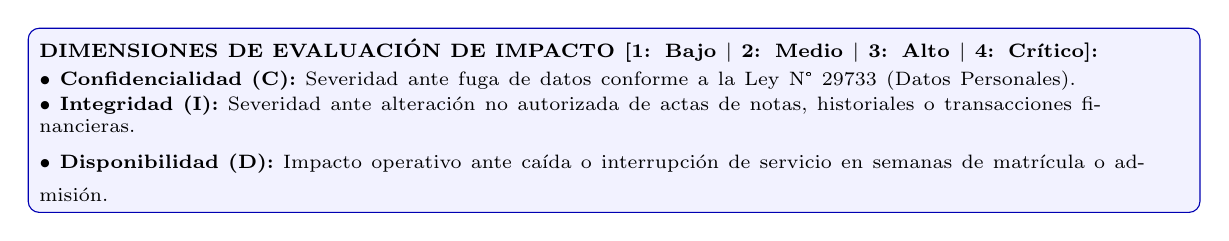
\begin{tikzpicture}[
    dimBox/.style={
        rectangle, rounded corners=4pt,
        inner sep=4pt, text width=14.6cm,
        draw=blue!70!black, fill=blue!5, align=left
    }
]
\node[dimBox] {
    {\bfseries\scriptsize DIMENSIONES DE EVALUACIÓN DE IMPACTO [1: Bajo $\vert$ 2: Medio $\vert$ 3: Alto $\vert$ 4: Crítico]:}\\[2pt]
    {\scriptsize $\bullet$ \textbf{Confidencialidad (C):} Severidad ante fuga de datos conforme a la Ley N° 29733 (Datos Personales).\\[1pt]
    $\bullet$ \textbf{Integridad (I):} Severidad ante alteración no autorizada de actas de notas, historiales o transacciones financieras.\\[1pt]
    $\bullet$ \textbf{Disponibilidad (D):} Impacto operativo ante caída o interrupción de servicio en semanas de matrícula o admisión.}
};
\end{tikzpicture}
\end{center}

\begin{center}
\scriptsize
\setlength{\tabcolsep}{3.5pt}
\renewcommand{\arraystretch}{1.2}
\begin{longtable}{>{\bfseries}c p{3.4cm} c c c c >{\bfseries}p{1.7cm} p{4.6cm}}
\toprule
\rowcolor{outermarginbgcolor}
ID & Activo Evaluado & C & I & D & Max & Criticidad & Justificación Operativa \\
\midrule
\endfirsthead
\toprule
\rowcolor{outermarginbgcolor}
ID & Activo Evaluado & C & I & D & Max & Criticidad & Justificación Operativa \\
\midrule
\endhead
\bottomrule
\endfoot
ACT-01 & Base de Datos Académica Central & 4 & 4 & 4 & 4 & Crítico & Alteración de notas o pérdida irreversible invalida semestres académicos. \\
\midrule
ACT-02 & Sistema de Matrícula (\texttt{matricula}) & 4 & 4 & 4 & 4 & Crítico & Punto único de fallo al inicio de semestre; expuesto a picos de denegación DoS. \\
\midrule
ACT-03 & Campus Virtual (\texttt{campus}) & 3 & 4 & 4 & 4 & Crítico & Soporte de evaluaciones en línea; su caída interrumpe labores formativas. \\
\midrule
ACT-04 & Enlaces WAN y Switch Core & 2 & 4 & 4 & 4 & Crítico & Su caída aísla la Ciudad Universitaria y sedes remotas de la UNAP. \\
\midrule
ACT-05 & Respaldo NAS (Inmutable) & 4 & 4 & 4 & 4 & Crítico & Último recurso de recuperación contra ransomware e incidentes destructivos. \\
\midrule
ACT-06 & Correo (\texttt{@unap.edu.pe}) & 4 & 3 & 3 & 4 & Alto & Identidad federada institucional; blanco directo de campañas Spear-Phishing. \\
\midrule
ACT-07 & Sistema de Trámite (SITRAD) & 3 & 4 & 3 & 4 & Alto & Afecta la validez legal y trazabilidad de decretos rectorales y resoluciones. \\
\midrule
ACT-08 & API de Marcación Biométrica & 3 & 3 & 2 & 3 & Alto & Contiene datos biométricos sensibles de trabajadores (Ley N° 29733). \\
\midrule
ACT-09 & Servidores de Dev (\texttt{dev}, \texttt{prue1}) & 3 & 2 & 1 & 3 & Alto (Riesgo) & Entornos vulnerables desactualizados que facilitan el movimiento lateral. \\
\midrule
ACT-10 & Repositorio Digital (DSpace) & 1 & 3 & 2 & 3 & Medio & Producción científica abierta; impacto reputacional si sufre desfiguración. \\
\bottomrule
\end{longtable}
\end{center}

% =============================================================================
% ANEXO 3
% =============================================================================
\newpage
\section*{Anexo 3: Matriz STRIDE y Evidencias Técnicas de Inspección}
\addcontentsline{toc}{section}{Anexo 3: Matriz STRIDE y Evidencias Técnicas de Inspección}

\subsection*{1. Ficha de Evidencia Técnica: Cabeceras y Cookies en matricula.unap.edu.pe}
\begin{itemize}[leftmargin=1.5em, itemsep=2pt]
    \item \textbf{Método de Extracción:} Inspección pasiva del cliente mediante navegador web (Herramientas DevTools F12 -- RFC 7230).
    \item \textbf{Endpoint Analizado:} \texttt{https://matricula.unap.edu.pe/matricula/alumno/}\\
    \texttt{horario?start=2026-10-12T00:00:00\&end=2026-10-18T00:00:00}
\end{itemize}

\begin{cmdbox}{Reporte de Captura DevTools: Cabeceras de Respuesta y Cookies}
HTTP/1.1 200 OK
Date: Sat, 17 Oct 2026 19:58:46 GMT
Content-Type: application/json; charset=utf-8
Transfer-Encoding: chunked
Connection: keep-alive
Server: nginx/1.16.1                                  <-- VULNERABILIDAD: Information Disclosure
Set-Cookie: .AspNetCore.Mvc.CookieTempDataProvider=;   <-- VULNERABILIDAD: Falta atributo 'Secure'
            expires=Thu, 01 Jan 1970 00:00:00 GMT; 
            path=/; samesite=lax; httponly

[COOKIES DE SESION IDENTIFICADAS EN EL CLIENTE]
- .AspNetCore.Cookies: Dividida en chunks (.AspNetCore.CookiesC1, .AspNetCore.CookiesC2)
- .AspNetCore.Mvc.CookieTempDataProvider: Estado temporal sin bandera Secure explicita
- AUSENCIA DE CABECERAS DEFENSIVAS:
  * Strict-Transport-Security (HSTS): NO PRESENTE (Riesgo SSL Stripping)
  * X-Frame-Options: NO PRESENTE (Riesgo Clickjacking)
  * Content-Security-Policy (CSP): NO PRESENTE (Riesgo XSS)
\end{cmdbox}

\subsection*{2. Matriz Operativa STRIDE Aplicada al Sistema de Matrícula}

\begin{center}
\scriptsize
\setlength{\tabcolsep}{3pt}
\renewcommand{\arraystretch}{1.2}
\begin{longtable}{>{\bfseries}p{1.9cm} p{1.9cm} p{4.0cm} >{\centering\arraybackslash}p{1.1cm} p{4.8cm}}
\toprule
\rowcolor{outermarginbgcolor}
Categoría & Elemento DFD & Hallazgo / Vulnerabilidad & Impacto & Contramedida Técnica Validada \\
\midrule
\endfirsthead
\toprule
\rowcolor{outermarginbgcolor}
Categoría & Elemento DFD & Hallazgo / Vulnerabilidad & Impacto & Contramedida Técnica Validada \\
\midrule
\endhead
\bottomrule
\endfoot
Spoofing & Flujo F-01 / Identidad & Ausencia de MFA obligatorio; persistencia de \texttt{.AspNetCore.Cookies} sin validación de IP. & Alto & Enrolamiento obligatorio en TOTP/FIDO2 y validación de huella TLS del cliente. \\
\midrule
Tampering & Límite 1 (Internet/DMZ) & HSTS ausente/desactivado; susceptible a ataques de SSL Stripping en redes Wi-Fi. & Alto & Inyección en Nginx: \texttt{add\_header Strict-Transport-Security "max-age=31536000; includeSubDomains; preload" always;}. \\
\midrule
Repudiation & Proceso P-04 / BD & Bitácoras sin registro atómico del User-ID en transacciones de cupos de horarios. & Medio & Logs inmutables (\textit{Append-Only}) centralizados en Syslog remoto con firma SHA-256. \\
\midrule
Information Disclosure & Proceso P-01 (Proxy) & Exposición de cabecera \texttt{Server: nginx/1.16.1} y cookies de ASP.NET Core. & Alto & Directiva \texttt{server\_tokens off;} en configuración de Nginx y actualización del paquete. \\
\midrule
Denial of Service & Proceso P-01 / API & Concurrencia masiva sin limitación de tasa en endpoint de consulta de horario. & Crítico & Directiva perimetral: \texttt{limit\_req zone=api\_matricula burst=25 nodelay;} (10 req/s por IP). \\
\midrule
Elevation of Privilege & Proceso P-03 / API & Control perimetral dependiente de URLs sin validación de roles en controladores backend. & Alto & Uso estricto de decoradores \texttt{[Authorize(Roles = "Docente,Admin")]} en ASP.NET Core. \\
\bottomrule
\end{longtable}
\end{center}

% =============================================================================
% ANEXO 4
% =============================================================================
\newpage
\section*{Anexo 4: Matriz MITRE ATT\&CK y Configuración de Reglas SIEM}
\addcontentsline{toc}{section}{Anexo 4: Matriz MITRE ATT\&CK y Configuración de Reglas SIEM}

\subsection*{1. Ficha de Mapeo de Técnicas Adversarias (UNAP)}

\begin{cmdbox}{Mapeo Institucional MITRE ATT\&CK Enterprise (UNAP)}
----------------------------------------------------------------------
          MAPEO INSTITUCIONAL MITRE ATT&CK ENTERPRISE (UNAP)
----------------------------------------------------------------------
TACTICA: Reconocimiento (TA0043)
- Tecnica: T1596.001 (Search Open Technical Databases: Certificates/crt.sh)
- Tecnica: T1589.002 (Gather Victim Identity Info: Email Addresses)

TACTICA: Acceso Inicial (TA0001)
- Tecnica: T1566.002 (Phishing: Spearphishing Link - Suplantacion)
- Tecnica: T1078.003 (Valid Accounts: Cuentas docentes sin segundo factor MFA)

TACTICA: Ejecucion (TA0002) y Persistencia (TA0003)
- Tecnica: T1059.001 (Command and Scripting: PowerShell en estaciones admin)
- Tecnica: T1505.003 (Server Software Component: Web Shell en directorios)

TACTICA: Movimiento Lateral (TA0008) y Exfiltracion (TA0010)
- Tecnica: T1021.002 (Remote Services: SMB/Windows Admin Shares inter-host)
- Tecnica: T1048.003 (Exfiltration Over Unencrypted Non-C2 Protocol)
----------------------------------------------------------------------
\end{cmdbox}

\subsection*{2. Evidencia de Implementación: Regla de Correlación para SIEM Wazuh}

\begin{cmdbox}{Regla Incorporada en /var/ossec/etc/rules/local\_rules.xml del SOC-UNAP}
<!-- Regla incorporada en el cluster SIEM Wazuh de la UNAP -->
<group name="unap_matricula,web_attack,">
  <!-- Deteccion de Intentos de Fuerza Bruta / Credential Stuffing -->
  <rule id="100201" level="10" frequency="10" timeframe="60">
    <if_matched_sid>31101</if_matched_sid>
    <url>/matricula/login|/auth/login</url>
    <description>ALERTA: Ataque fuerza bruta en portal matricula (T1110)</description>
    <mitre>
      <id>T1110.001</id>
    </mitre>
    <action>firewall-drop</action>
  </rule>
</group>
\end{cmdbox}

% =============================================================================
% ANEXO 5
% =============================================================================
\newpage
\section*{Anexo 5: Cyber Kill Chain y Evidencias de Configuración DNS}
\addcontentsline{toc}{section}{Anexo 5: Cyber Kill Chain y Evidencias de Configuración DNS}

\subsection*{1. Ficha de Evidencia Técnica de Consultas DNS (Terminal de Comandos)}
\begin{itemize}[leftmargin=1.5em, itemsep=2pt]
    \item \textbf{Herramienta Empleada:} \texttt{nslookup} sobre servidores DNS públicos (Resolución no autoritativa).
    \item \textbf{Fecha de Extracción:} Octubre 2026.
\end{itemize}

\begin{cmdbox}{Consultas DNS sobre el Dominio unap.edu.pe}
[CONSULTA REGISTRO SPF: unap.edu.pe]
$ nslookup -type=TXT unap.edu.pe
unap.edu.pe   text = "v=spf1 ip4:208.70.245.162 a:sfulib10.nmsrv.com include:_spf.google.com ~all"
DIAGNOSTICO: Directiva finaliza en ~all (SoftFail). Los servidores de correo 
             receptores no descartan correos apocrifos.

[CONSULTA REGISTRO DMARC: _dmarc.unap.edu.pe]
$ nslookup -type=TXT _dmarc.unap.edu.pe
*** ns47.wowperu.pe no encuentra _dmarc.unap.edu.pe: Non-existent domain
DIAGNOSTICO: NXDOMAIN (Inexistente). La universidad no tiene politica de proteccion 
             contra suplantacion de dominio. Brecha critica en Kill Chain Fase 3.
\end{cmdbox}

\subsection*{2. Matriz de Ruptura de la Kill Chain en la UNAP}

\begin{center}
\small
\setlength{\tabcolsep}{4pt}
\renewcommand{\arraystretch}{1.2}
\begin{longtable}{>{\bfseries}p{4.2cm} p{10.2cm}}
\toprule
\rowcolor{outermarginbgcolor}
Fase de la Cyber Kill Chain & Control Técnico Clave de Ruptura Defensiva \\
\midrule
\endfirsthead
\toprule
\rowcolor{outermarginbgcolor}
Fase de la Cyber Kill Chain & Control Técnico Clave de Ruptura Defensiva \\
\midrule
\endhead
\bottomrule
\endfoot
FASE 1: Reconocimiento & Directiva \texttt{server\_tokens off;} en Nginx y baja de subdominios de prueba (\texttt{dev}, \texttt{prue1}). \\
\midrule
FASE 2: Armamento & Monitoreo activo de Threat Intelligence sobre registros DNS y certificados con typosquatting. \\
\midrule
FASE 3: Entrega & \textbf{Control Clave:} Publicación de directiva DMARC (\texttt{p=reject}) y política SPF restrictiva (\texttt{-all}). \\
\midrule
FASE 4: Explotación & Habilitación obligatoria de HSTS con flag \texttt{preload} y actualización de software desactualizado. \\
\midrule
FASE 5: Instalación & \textbf{Control Clave:} MFA obligatorio en VPN e Intranet, con despliegue de agentes EDR en servidores. \\
\midrule
FASE 6: Comando y Control (C2) & Filtrado de salida (\textit{Egress Filtering}) en NGFW, bloqueando puertos y protocolos no autorizados. \\
\midrule
FASE 7: Acciones sobre Objetivos & Microsegmentación en VLAN 10 (BD aislada) y almacenamiento de respaldos inmutables 3-2-1 WORM. \\
\bottomrule
\end{longtable}
\end{center}

% =============================================================================
% ANEXO 6
% =============================================================================
\vspace{0.4cm}
\section*{Anexo 6: Matriz Zero Trust y Evidencias de Postura TLS}
\addcontentsline{toc}{section}{Anexo 6: Matriz Zero Trust y Evidencias de Postura TLS}

\subsection*{1. Ficha de Evidencia: Negociación TLS en campus.unap.edu.pe}
\begin{itemize}[leftmargin=1.5em, itemsep=2pt]
    \item \textbf{Método:} Inspección del handshake criptográfico en navegador web cliente.
\end{itemize}

\begin{cmdbox}{Reporte de Seguridad TLS: campus.unap.edu.pe}
[REPORTE DE SEGURIDAD TLS: campus.unap.edu.pe]
Version del Protocolo:     TLSv1.2 (Soporte pendiente para TLSv1.3 estandar Zero Trust)
Suite de Cifrado:          TLS_ECDHE_RSA_WITH_AES_128_GCM_SHA256
HSTS (Transporte Seguro):  "Desactivado" (Vulnerabilidad critica MitM)
Certificado Digital:       Let's Encrypt (Rango validez: Sat, 19 Sep 2026 - Fri, 18 Dec 2026)
Pinning de Clave Publica:  Desactivado
\end{cmdbox}

\subsection*{2. Esquema de Segmentación de Red y Matriz de Control de Accesos}

\begin{center}
\begin{tikzpicture}[
    scale=0.92, transform shape,
    boxExt/.style={rectangle, rounded corners=3pt, draw=gray!70, fill=gray!10, text width=7cm, align=center, font=\footnotesize\bfseries, inner sep=4pt},
    boxWAF/.style={rectangle, rounded corners=3pt, draw=blue!75!black, fill=blue!10, text width=5.5cm, align=center, font=\footnotesize\bfseries, inner sep=5pt},
    boxVLAN/.style={rectangle, rounded corners=4pt, draw=teal!80!black, fill=teal!8, text width=4.8cm, align=center, font=\scriptsize, inner sep=5pt},
    boxDC/.style={rectangle, rounded corners=4pt, draw=red!75!black, fill=red!6, text width=11.5cm, align=center, font=\scriptsize, inner sep=6pt},
    conn/.style={-{Stealth[scale=0.85]}, line width=1.1pt, color=fg!80!black}
]

\node[boxExt] (ext) at (0, 4.2) {INTERNET / USUARIOS EXTERNOS};
\node[boxWAF] (waf) at (0, 2.9) {WAF / NGFW FortiGate};

\node[boxVLAN] (v60) at (-3.6, 1.2) {
    {\bfseries\color{teal!80!black} VLAN 60 -- DMZ Portales}\\[2pt]
    Portales Web Públicos\\
    (\texttt{matricula}, \texttt{campus}, \texttt{admision})
};

\node[boxVLAN] (v50) at (3.6, 1.2) {
    {\bfseries\color{teal!80!black} VLAN 50 -- Wi-Fi Campus}\\[2pt]
    Redes Inalámbricas e Invitados\\
    (Salida exclusiva a Internet)
};

\node[boxDC] (v10) at (0, -1.0) {
    {\bfseries\color{red!75!black} VLAN 10 -- Data Center Crítico (Base de Datos + Backups NAS Inmutables)}\\[2pt]
    $\bullet$ Acceso desde VLAN 60: Túnel SQL controlado y estricto (\textbf{solo TCP 5432 / 1521}).\\
    $\bullet$ Acceso Administrativo: Exclusivo mediante Bastión Jump Host con mTLS y MFA.
};

\draw[conn] (ext) -- (waf);
\draw[conn] (waf.south) -- ++(0,-0.3) -| (v60.north);
\draw[conn] (waf.south) -- ++(0,-0.3) -| (v50.north);
\draw[conn] (v60.south) -- node[left, font=\tiny\bfseries] {Solo TCP 5432} (v60.south |- v10.north);

\end{tikzpicture}
\end{center}

% =============================================================================
% ANEXO 7
% =============================================================================
\newpage
\section*{Anexo 7: Formato Oficial de Registro y Control de Incidentes}
\addcontentsline{toc}{section}{Anexo 7: Formato Oficial de Registro y Control de Incidentes}

\begin{cmdbox}{CSIRT-UNAP: Hoja Oficial de Registro y Control de Incidente}
----------------------------------------------------------------------
     OFICINA DE TECNOLOGIAS DE LA INFORMACION - CSIRT UNAP
         HOJA DE REGISTRO DE INCIDENTE DE SEGURIDAD DIGITAL
----------------------------------------------------------------------
CODIGO DE SEGUIMIENTO: INC-UNAP-2026-________  FECHA: __/__/2026  HORA: __:__
RESPONSABLE DE ATENCION: ____________________  ESTADO: [ ] Abierto [ ] Analisis
PRIORIDAD: [ ] Nivel 1 (Baja)   [ ] Nivel 2 (Media)    [ ] Contenido [ ] Cerrado
           [ ] Nivel 3 (Alta)   [ ] Nivel 4 (Critica)

1. TIPO DE AMENAZA:
   [ ] Suplantacion de Dominio / Phishing        [ ] DoS / DDoS
   [ ] Infeccion Malware / Ransomware            [ ] Intrusion Web / Web Shell
   [ ] Acceso con Cuentas Validas Robadas        [ ] Fuga Datos (Ley 29733)

2. ACTIVOS Y ENTORNOS COMPROMETIDOS:
   Nombre Activo: ___________________________ IP / Subdominio: _______________
   VLAN: [ ] VLAN 10 (BD)  [ ] VLAN 20 (Doc)  [ ] VLAN 30 (Adm)  [ ] VLAN 60

3. VECTOR DE ENTRADA Y DESCRIPCION TECNICA:
   ___________________________________________________________________
   ___________________________________________________________________

4. EVIDENCIAS RECOLECTADAS (IoCs):
   IPs Atacantes: ___________________________ Hashes: ________________
   URLs / Dominios: _________________________ Cuentas: _______________

5. TIEMPOS OPERATIVOS DE RESPUESTA:
   Hora Detec.: ____:____  Hora Contenc.: ____:____  MTTD: ___ min  MTTR: ___ min

6. ACCIONES DE RECUPERACION Y FIRMAS:
   [ ] Restauracion Copia Inmutable (3-2-1)   [ ] Parche Hardening Nginx/DMARC
   Se notifico al CSIRT Nacional (PCM)?: [ ] SI  [ ] NO   Fecha: ____/____/2026

   ____________________________________   ____________________________________
   Firma Oficial de Seguridad (CISO)      Firma Administrador Redes/Sistemas
----------------------------------------------------------------------
\end{cmdbox}

% =============================================================================
% ANEXO 8
% =============================================================================
\newpage
\section*{Anexo 8: Cronograma Anual de Implementación y Despliegue (Gantt)}
\addcontentsline{toc}{section}{Anexo 8: Cronograma Anual de Implementación y Despliegue (Gantt)}

Planificación estructurada a doce (12) meses para la ejecución escalonada de controles técnicos y adecuación institucional en la UNAP:

\begin{center}
\scriptsize
\setlength{\tabcolsep}{2.5pt}
\renewcommand{\arraystretch}{1.15}
\begin{longtable}{p{4.5cm} *{12}{>{\centering\arraybackslash}p{0.53cm}} p{3.2cm}}
\toprule
\rowcolor{outermarginbgcolor}
Tarea / Hito Operativo & M1 & M2 & M3 & M4 & M5 & M6 & M7 & M8 & M9 & M10 & M11 & M12 & Responsable Directo \\
\midrule
\endfirsthead
\toprule
\rowcolor{outermarginbgcolor}
Tarea / Hito Operativo & M1 & M2 & M3 & M4 & M5 & M6 & M7 & M8 & M9 & M10 & M11 & M12 & Responsable Directo \\
\midrule
\endhead
\bottomrule
\endfoot
\multicolumn{14}{l}{\bfseries\color{blue!75!black} Fase 1: Corrección Perimetral y DNS} \\
\midrule
Publicación DMARC (\texttt{p=reject}) y SPF (\texttt{-all}) & $\bullet$ & & & & & & & & & & & & OTI / Unidad de Redes \\
Hardening Nginx (HSTS, \texttt{server\_tokens off;}) & $\bullet$ & $\bullet$ & & & & & & & & & & & OTI / Webmaster \\
Baja de subdominios \texttt{dev}/\texttt{prue1} expuestos & $\bullet$ & & & & & & & & & & & & OTI / Sistemas \\
\midrule
\multicolumn{14}{l}{\bfseries\color{blue!75!black} Fase 2: Identidad y Zero Trust} \\
\midrule
Despliegue MFA obligatorio (Docentes y Admin) & & $\bullet$ & $\bullet$ & $\bullet$ & & & & & & & & & OTI / Gestión Identidades \\
Microsegmentación de VLANs en Core Switch & & $\bullet$ & $\bullet$ & $\bullet$ & & & & & & & & & OTI / Unidad de Redes \\
Implementación de flag Secure en cookies ASP.NET & & $\bullet$ & $\bullet$ & & & & & & & & & & Desarrolladores OTI \\
\midrule
\multicolumn{14}{l}{\bfseries\color{blue!75!black} Fase 3: Monitoreo y SOC Institucional} \\
\midrule
Despliegue de Wazuh SIEM y agentes EDR & & & & $\bullet$ & $\bullet$ & $\bullet$ & & & & & & & SOC / Redes \\
Configuración de reglas detección MITRE ATT\&CK & & & & & $\bullet$ & $\bullet$ & & & & & & & Analista Ciberseguridad \\
Ingesta de Threat Intelligence y MISP institucional & & & & & $\bullet$ & $\bullet$ & & & & & & & Analista Ciberseguridad \\
\midrule
\multicolumn{14}{l}{\bfseries\color{blue!75!black} Fase 4: Continuidad y Factor Humano} \\
\midrule
Configuración de Backups Inmutables (WORM 3-2-1) & & & & & & $\bullet$ & $\bullet$ & & & & & & Administrador de BD \\
Primer Simulacro de Restauración de BD Académica & & & & & & & $\bullet$ & & & & & & DBA / OTI \\
Campaña 1 de Phishing Simulado (Personal) & & & $\bullet$ & & & & & & & & & & CISO / Recursos Humanos \\
Campaña 2 de Phishing Simulado (Personal) & & & & & & & & & $\bullet$ & & & & CISO / Recursos Humanos \\
Taller Anual de Ciberseguridad Docente & & & & & & & & & $\bullet$ & $\bullet$ & & & Recursos Humanos / OTI \\
Auditoría Anual y Revisión NIST CSF 2.0 & & & & & & & & & & & $\bullet$ & $\bullet$ & CISO / Rectorado \\
\bottomrule
\end{longtable}
\end{center}

% =============================================================================
% ANEXO 9
% =============================================================================
\newpage
\section*{Anexo 9: Cuadro de Mando de Indicadores de Ciberseguridad (KPIs)}
\addcontentsline{toc}{section}{Anexo 9: Cuadro de Mando de Indicadores de Ciberseguridad (KPIs)}

Plantilla consolidada de seguimiento y control directivo con el estado de avance sobre la línea base identificada en la auditoría inicial de la UNAP:

\begin{cmdbox}{UNAP: Dashboard Ejecutivo de Ciberseguridad 2026}
----------------------------------------------------------------------
             UNAP | DASHBOARD EJECUTIVO DE CIBERSEGURIDAD 2026
----------------------------------------------------------------------
INDICADOR (KPI)                 FORMULA              META   BASE  ESTADO
----------------------------------------------------------------------
KPI-01: Cobertura Inventario    (A_inv / A_tot)*100  >=98%   65%  EN PROCESO
KPI-02: Cobertura STRIDE        (S_eval / S_crit)*100 100%   20%  EN PROCESO
KPI-03: Remediacion Vuln.       (V_corr / V_det)*100 >=90%   40%  CRITICO
KPI-04: Adopcion MFA Personal   (U_mfa / U_req)*100   100%   15%  CRITICO
KPI-05: Vulnerabilidad Phish.   (U_click / U_dest)*100 <=8%  38%  EN RIESGO
KPI-06: Capacitacion Personal   (P_cert / P_tot)*100 >=85%   10%  PLANIFICADO
KPI-07: Tiempo Deteccion (MTTD) Promedio(T_det - T_0)<=120m  48h  CRITICO
KPI-08: Tiempo Respuesta (MTTR) Promedio(T_cont-T_det)<=60m  12h  CRITICO
KPI-09: Fiabilidad de Backups   (R_exit / R_ejec)*100 100%  100%  CUMPLIDO
KPI-10: Rechazo DMARC           (C_rech / C_fals)*100 >=99%   0%  CRITICO
----------------------------------------------------------------------
\end{cmdbox}

% =============================================================================
% ANEXO 10
% =============================================================================
\newpage
\section*{Anexo 10: Plan y Malla Curricular de Capacitación Institucional}
\addcontentsline{toc}{section}{Anexo 10: Plan y Malla Curricular de Capacitación Institucional}

Programa formativo anual de carácter obligatorio y certificable para los diferentes estamentos de la comunidad universitaria:

\begin{center}
\scriptsize
\setlength{\tabcolsep}{3pt}
\renewcommand{\arraystretch}{1.2}
\begin{longtable}{>{\bfseries}p{1.1cm} p{2.5cm} p{4.3cm} >{\centering\arraybackslash}p{1.3cm} p{2.1cm} p{2.6cm}}
\toprule
\rowcolor{outermarginbgcolor}
Módulo & Público Objetivo & Contenido Temático Específico & Duración & Modalidad & Criterio de Evaluación \\
\midrule
\endfirsthead
\toprule
\rowcolor{outermarginbgcolor}
Módulo & Público Objetivo & Contenido Temático Específico & Duración & Modalidad & Criterio de Evaluación \\
\midrule
\endhead
\bottomrule
\endfoot
M-01 & Comunidad Estudiantil (Pregrado y Posgrado) & $\bullet$ Identificación de dominios falsos (\texttt{matricula-unap\dots}). \newline $\bullet$ Peligros al usar redes Wi-Fi públicas abiertas. \newline $\bullet$ Procedimiento de reporte al buzón institucional. & 2 horas & Virtual Asíncrono (Campus Virtual) & Cuestionario interactivo (Nota aprobatoria mín.\ 14). \\
\midrule
M-02 & Plana Docente (20 Facultades) & $\bullet$ Enrolamiento y uso de aplicaciones MFA (TOTP). \newline $\bullet$ Custodia de actas de notas y expedientes. \newline $\bullet$ Prevención de ataques de ingeniería social y phishing. & 4 horas & Semipresencial / Talleres OTI & Simulación práctica en aula virtual institucional. \\
\midrule
M-03 & Personal Administrativo (Caja, RRHH, SITRAD) & $\bullet$ Tratamiento de datos personales (Ley N° 29733). \newline $\bullet$ Política de puestos limpios y bloqueo de pantalla. \newline $\bullet$ Prevención de infecciones cruzadas por memorias USB. & 4 horas & Presencial por Facultades & Auditoría sorpresa en puesto de trabajo. \\
\midrule
M-04 & Desarrolladores y Programadores OTI & $\bullet$ Codificación segura (Estándares OWASP Top 10). \newline $\bullet$ Hardening de APIs en ASP.NET Core y cookies seguras. \newline $\bullet$ Gestión de secretos y uso de Git sin credenciales. & 16 horas & Taller Teórico-Práctico intensivo & Análisis estático de código (SAST) en proyectos activos. \\
\midrule
M-05 & Administradores de Red y Sistemas OTI & $\bullet$ Hardening de proxies Nginx y servidores Linux/Windows. \newline $\bullet$ Monitoreo, creación de reglas Wazuh e ingesta de CTI. \newline $\bullet$ Protocolos de respuesta a incidentes del CSIRT-UNAP. & 20 horas & Especializado (Laboratorio Forense) & Ejercicio de simulación \textit{Tabletop} ante brecha real. \\
\bottomrule
\end{longtable}
\end{center}